\documentclass{ctexart}
\usepackage{geometry}
\usepackage{diagbox}
\usepackage{graphicx}
\usepackage{subfigure}
\usepackage{amsmath}
\usepackage{amssymb}
\usepackage{indentfirst}
\usepackage{xfrac}
\usepackage{color}
\usepackage[table]{xcolor}
\usepackage{multirow}
\usepackage{titlesec}
\usepackage{bm}
\usepackage{caption}
\title{基于LSTM的风力系统上网功率预测}
\author{未央-能动02\quad 徐智昱\quad 2020012991}
\date{}
\begin{document}
\maketitle
\begin{abstract}
    在双碳目标下,根据历史数据对风电机未来一段时间内的运行状况结合其它设施进行调峰具有重大意义。本研究采用实际获得的风电机组一个月的运行数据
    与当地一个月的风力数据,进行未来1小时每15分钟一个点的功率预测。风电机的功率与当地风速有着紧密关系,而风速与风功率也有明显的自回归现象,
    因此考虑能够考虑这种自回归与相关性的模型进行建模。循环神经网络(RNN)就是这样一种方法,本研究采用了长短期记忆网络(LSTM)对风功率的预测进行了研究,
    并通过调整参数试图找到较为适合的模型。同时,也考虑利用传统的时间序列分析(TSA)的方法对此数据进行考量,比较经典方法与现代方法之间效果的差异。
\end{abstract}
\textbf{关键词:} TSA, RNN, LSTM
\section{引言}
\subsection{数据描述与预处理}
获得的风电数据来自江苏的风电场,包含风速与风功率两组变量,在2015/10/1 0:00到2015/10/31 23:59被采集,每30秒采集一次数据,
内有一系列缺失数据。根据国家标准,需要对未来1个小时的4个,每个间隔15分钟的点进行预测,因此将数据集每15个点进行合并,可以借此作出散点图
与时序图。\\
\begin{figure}[htbp]
    \centering
    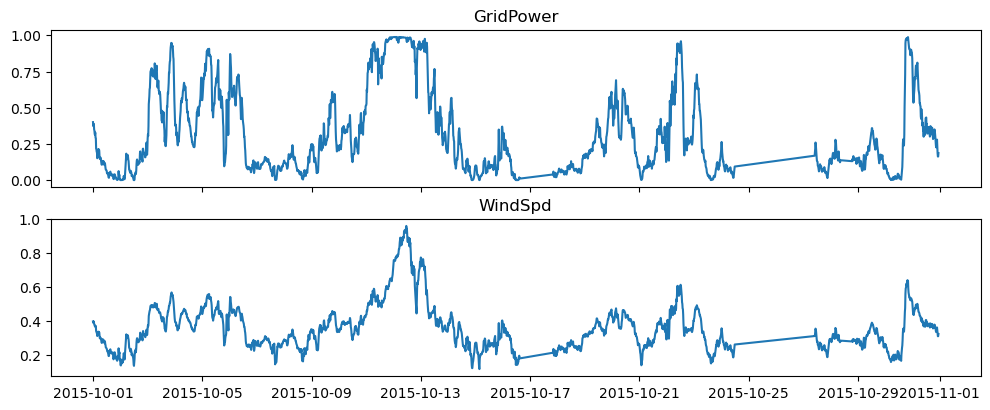
\includegraphics[width=0.80\textwidth]{photos/original_time_series.png}
    \caption{原始数据时序图}
\end{figure}
由时序图可以发现其存在较多的时间缺失区间,因此在实际建立模型时选择使用分段的区间进行模型的训练,放弃具有缺失值的部分。\\
\indent 同时可以作出的风功率与风速关系的图像,并同时用Kernel Regression对数据符合的形式作初步的拟合,结果如下图所示:\\
\begin{figure}[htbp]
    \centering
    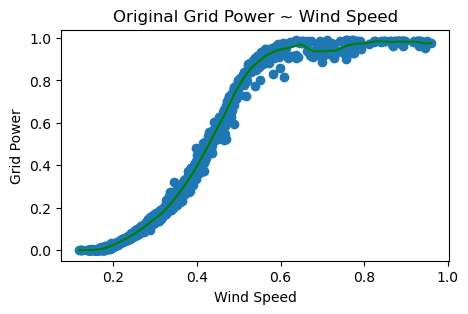
\includegraphics[width = 0.6\textwidth]{photos/scatter_fitted.png}
    \caption{风功率风速关系图}
\end{figure}
由图可见,二者关系可能近似符合类似于Logistic Function的形式;同时可能经过恰当的变换后,可以找到用于描述的线性函数描述其变化。\\
\indent 在时间序列中,常用的检测离群值(Outlier)的方法是认为每个数据独立同分布地服从于正态分布,由正态分布的置信区间判断有无明显的离群值。
利用这个方法可以作出此数据的离群值:\\
\begin{figure}[htbp]
    \centering
    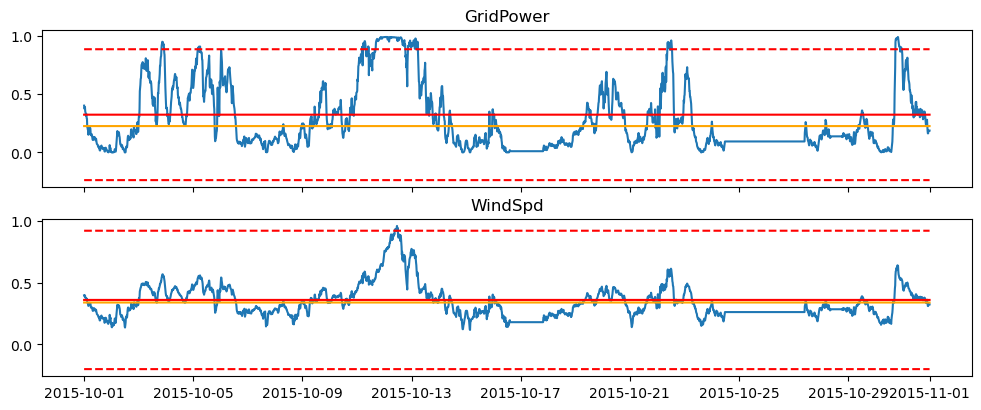
\includegraphics[width=0.80\textwidth]{photos/outliers.png}
    \caption{离群值检测}
\end{figure}
由图像可以发现,数据的特性良好,存在极少的离群值,因此不需要对数据的离群值进行处理。\\
\indent 由图1可见,数据实际上存在较多的噪音,因此考虑使用滑动平均(Moving Average)的方法,降低数据的噪音。下图是以20个数据点为窗口的滑动平均的结果:\\
\begin{figure}[htbp]
    \centering
    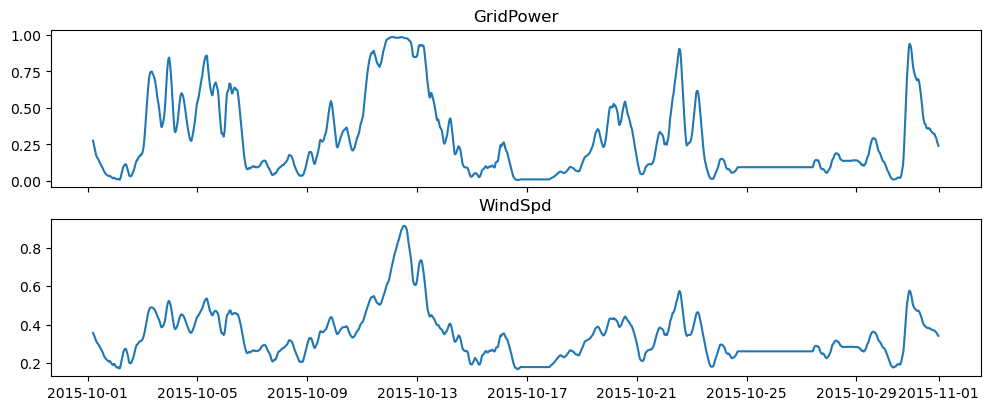
\includegraphics[width = 0.8\textwidth]{photos/ma_time_series.png}
    \caption{滑动平均数据}
\end{figure}
滑动平均后数据明显变得光滑,但也失去了一部分的信息,将对滑动平均前后分别建立模型进行研究来探究实际中应该使用何种模型进行
训练。\\

\subsection{方法概述}
在进行模型的选择前,首先对能够利用的方法进行了调研,通过课上学习与课外阅读,了解学习了以下方法,并对其中一些方法进行了试验
与调参。\\
\indent 本文遇到的序列是时间序列数据,其突出特点为具有强时空相关性,有明显的自回归效应,通过作出其自回归(autocorrelation)图
可见一斑。其自回归图如图所示:\\
\begin{figure}[htbp]
    \centering
    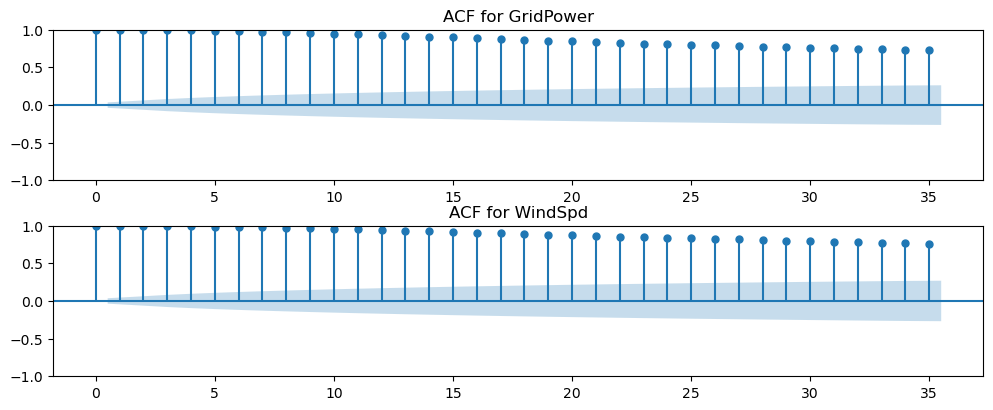
\includegraphics[width=0.8\textwidth]{photos/acf.png}
    \caption{ACF for GridPower and WindSpd}
\end{figure}
\indent 因此在方法的选择中,应注意选择使用能够考虑到时空自相关性的方法;这意味着纯粹的线性回归(Linear Regression)模型
对此数据就预测4个点意义上应不具有良好的效果。经过调研,对以下方法进行了研究学习。
\subsection{隐马尔可夫模型(HMM)}
本次获得的时间序列,在物理意义上可以看作变量风速(WindSpd)对风能(GridPower)有一个因果的作用。由探索性数据分析,也可看到
二者之间存在比较良好的关系(图2)。因此,可以认为二者之间服从于一个条件分布的关系,条件于过去一段时间的自身的数值与自变量的数值。
为书写简便,将风能(GridPower)记为$Y$,
将风速(WindSpd)记为$X$。
\begin{equation*}
    Y_n \sim P(Y_n|y_1,y_2,\cdots,y_{n-1},x_1,x_2,\cdots,x_n)
\end{equation*}
由上式可以发现,若考虑全序列对该点的影响,模型会非常复杂,并且计算上非常耗费时间与精力。因此在实际中经常引入马尔可夫性质(Markov Property),即
因变量只由该时间的自变量影响,而自变量仅由上一个时间点的自变量决定。即
\begin{align*}
    P(Y_n|y_1,y_2,\cdots,y_{n-1},x_1,x_2,\cdots,x_n) &= P(Y_n|x_n)\\
    P(X_n|x_1,x_2,\cdots,x_{n-1}) &= P(X_n|x_{n-1}) 
\end{align*}
可以看出这对模型作了非常大的简化,在实际运行中很多时候也能达成较好的效果。\\
\indent HMM主要运用于离散态的过程,对于本次的连续类型数据,也可以有HGMM(Hidden Gauss Markov Model)等变体,即
将马尔可夫矩阵变成特定类型分布,对数据进行参数的学习,通过MLE(Maximum Likelihood Estimation)等方式产生点估计。\\
\indent 接下来,可以用EM算法对数据进行迭代学习,从而达到收敛;或者通过贝叶斯的方法通过MCMC进行参数估计。\\
\indent 由于马尔可夫模型具有良好的概率性质,因此非常方便地能够得到估计的置信区间等统计量,从而比较方便地
判断估计的准确程度。然而对于比较复杂的数据,比如本文用到的数据,预测的效果可能不那么好。因此本文将不采用
HMM进行数据的分析。
\subsubsection{LSTM}
循环神经网络(RNN)可以很好地处理序列信息,通过引入状态变量存储过去的信息和当前的输入,从而确定当前的
输出。\\
\indent RNN的本质是一种自回归模型,认为当前值具有某种意义上的马尔可夫性质,其概率分布只与过去一段时间
的数据点相关,因此通过观察一个非常短的历史就能够预测未来的情况如何。由于在实际中,时间较为久远的信息
对当前的影响一般会随时间减小,因此经常可以忽略不计。RNN加入了和马尔可夫模型类似的隐变量,
对过去一段时间的输入进行保存,从而学习出模型。\\
\indent RNN模型的结构如图所示,其中$x$为输入层,$h$为隐藏层,$y$为输出层。\\
\begin{figure}[htbp]
    \centering
    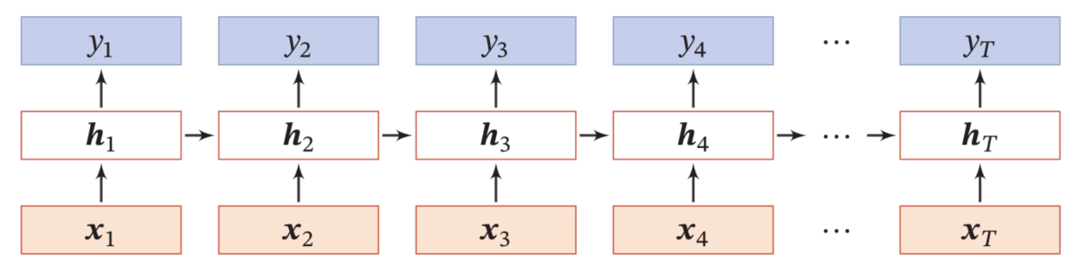
\includegraphics[width=0.70\textwidth]{photos/RNN.png}
    \caption{RNN结构概念图}
\end{figure}
\indent 在RNN模型中,利用迭代的方法对模型进行优化,在实际使用中使用batch的方法,采用Stochastic Graident 
Descent利用梯度下降的方法对模型参数进行优化,从而得到在loss function意义下具有优越性的模型。为了提高模型
的鲁棒性,又提出了LSTM模型。\\
\indent 由于隐变量模型存在着长期信息保存和短期输入缺失的问题,长短期记忆网络(LSTM)引入了计算机的逻辑门,
其中一个门用来输出,另一哥们用来决定何时读入,并增加控制何时对单元进行重置的门。三个门都利用线性运算与
隐藏层相关联。通过三个门的状态不同,决定LSTM在不同时刻的计算状态,从而实现对过去数据的记忆与以往的过程,
达到比较良好的效果。\\
\indent LSTM模型的结构如图所示\\
\begin{figure}
    \centering
    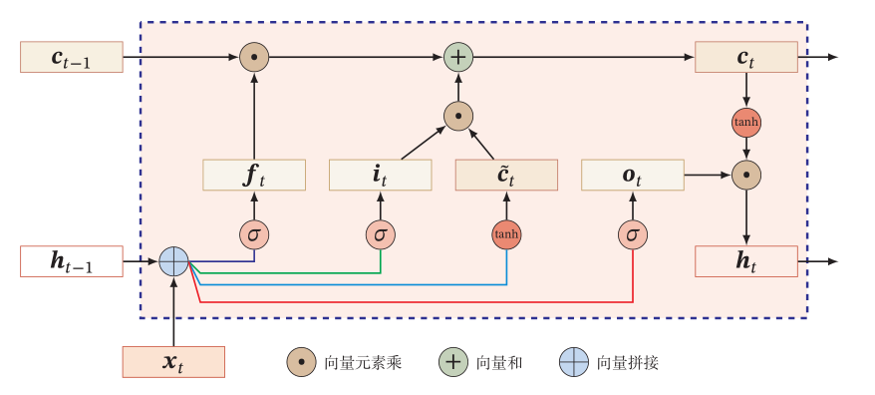
\includegraphics[width=0.70\textwidth]{photos/LSTM.png}
    \caption{LSTM结构概念图}
\end{figure}
其原理为:
\begin{enumerate}
    \item [(1)] 首先利用上一个时刻的外部状态$h_{t-1}$和当前时刻的输入$x_t$计算出三个门以及候选状态$\tilde{c}_t$。
    \item [(2)] 结合遗忘门$f_t$和输入们$i_t$更新记忆单元$c_t$。
    \item [(3)] 结合输出门$o_t$将内部信息传递给外部状态$h_t$
\end{enumerate}
\indent 由于LSTM天然地具有良好的处理时空相关性的能力,因此本文采用LSTM进行部分的研究。
\subsection{评价指标}
本文采用MSE和Qualification Rate两个指标对不同模型得到的结果进行评价。二者定义分别如下。\\
\begin{equation}
    MSE = \sqrt{\frac{1}{n}\sum_{i=1}^n (y_i-\hat{y}_i)^2}
\end{equation}
\begin{equation}
    Q = \frac{1}{n}\sum_{i=1}^n B_i\times 100\%
\end{equation}
\begin{equation}
    B_i = \left\{
        \begin{aligned}
            &1, 1-|y_i-\hat{y}_i \geq 0.85\\
            &0, 1-|y_i-\hat{y}_i| < 0.85
        \end{aligned}
        \right .
\end{equation}
其中$y_i$为序列中第$i$项的真值,$\hat{y}_i$为序列中第$i$项的预测值。MSE可以用来表征数据的预测程度的好坏,
MSE越小代表预测值与真值在均方误差意义下更加接近。Q则为观测预测值符合国家标准的数量,更直观地观测预测方法的好坏。

\section{主要内容}
\subsection{LSTM的参数调节}
在LSTM的参数的训练中,本文采用了输入一个序列中的风功率和风速的历史点,预测序列结束后4个点的方式对未来结果进行预测。因此,在参数设定中,
选择将输入大小选为2,分别代表着过去一段时间的风功率和风速的输入,输出大小为4,代表着预测接下来4个时间点的风功率大小。在训练集和测试集的选取中,
由于每一段不间断的部分均较长,能够作为输入进入LSTM的模型中,而经过尝试,使用的各种填补方法(具体见期中作业)效果均不尽如人意,可能会造成
数据信息量的损失,因此不对数据进行填补。由前期的数据分析可以得知,在数据集中能够利用的数据可以分为4部分,按时间顺序为叙述简便分别在下文称为
数据集1、2、3、4,在本处,将数据集1、2、3作为训练集,将数据集4作为测试集,进行数据的处理。\\
在LSTM的运行中,具有重要作用的参数主要有输入序列的长度、隐含层的节点数量、隐含层的层数、batch的大小,

\section{结论}

\section{参考文献}
\noindent [1] 邱锡鹏,神经网络与深度学习,机械工业出版社,https://nndl.github.io/, 2020.\\
\noindent [2] William Turin, Springer US, Performance Analysis and Modeling of Digital Transmission Systems, Continuous State HMM, 2004\\
\noindent [3] 
\end{document}